\documentclass[14pt]{article}
\usepackage[utf8]{inputenc}
\usepackage[T2A]{fontenc}
\usepackage[russian]{babel} % Кириллица uchun, lekin matn lotin yozuvida
\usepackage{amsmath, amssymb}
\usepackage{geometry}
\usepackage{graphicx}
\usepackage{xcolor}
\usepackage{hyperref}
\usepackage{tasks}
\usepackage{tcolorbox}
\tcbuselibrary{skins, breakable, theorems}
\usepackage{fancyhdr}
\usepackage{lastpage}
\usepackage{enumitem}
\usepackage{paracol}
\usepackage{ifthen}
\usepackage{needspace}

% Определение команд для тангенса и котангенса (русский стиль)
\newcommand{\tg}{\operatorname{tg}}
\newcommand{\ctg}{\operatorname{ctg}}

% Настройка геометрии
\geometry{a4paper, left=10mm, right=10mm, top=20mm, bottom=20mm, headheight=15pt}

% Цветовая палитра
\definecolor{primary}{RGB}{52, 152, 219}
\definecolor{secondary}{RGB}{46, 204, 113}
\definecolor{accent}{RGB}{155, 89, 182}
\definecolor{lightbg}{RGB}{248, 249, 250}
\definecolor{taskborder}{RGB}{230, 230, 230}
\definecolor{optionbg}{RGB}{240, 242, 245}

% Основной фон страницы
\pagecolor{lightbg}

% Настройка гиперссылок
\hypersetup{
    colorlinks=true,
    linkcolor=primary,
    urlcolor=primary,
}

% Колонтитулы
\pagestyle{fancy}
\fancyhf{}
\fancyhead[L]{\textcolor{primary}{\textbf{MathCore | MOCK Test-9}}}
\fancyhead[R]{\textcolor{secondary}{Abdunazarov M.X.}}
\fancyfoot[L]{\href{https://t.me/Math_Core_Dtm_MS_Att}{\textcolor{primary}{MathCore}}}
\fancyfoot[R]{\href{https://t.me/Abd_mardon}{\textcolor{secondary}{@Abd\_mardon}}}
\fancyfoot[C]{\textcolor{gray}{\thepage/\pageref{LastPage}}}
\renewcommand{\headrulewidth}{0.5pt}
\renewcommand{\headrule}{\hbox to\headwidth{\color{primary}\leaders\hrule height \headrulewidth\hfill}}
\renewcommand{\footrulewidth}{0.5pt}
\renewcommand{\footrule}{\hbox to\headwidth{\color{secondary}\leaders\hrule height \footrulewidth\hfill}}

% Титульная страница
\title{\Huge \textbf{\textcolor{primary}{MOCK Test-9}}}
\author{\textcolor{secondary}{Abdunazarov M.X.}}
\date{}
\newenvironment{сc}{\begin{center}}{\end{center}}
% Стиль для карточки вопроса
\newtcolorbox{questionbox}[2][]{
    enhanced,
    breakable,
    colback=white,
    colframe=primary,
    coltitle=white,
    fonttitle=\bfseries\large,
    title={Задача \hfill \textcolor{white}{#2}},
    attach boxed title to top left={xshift=5mm, yshift=-2mm},
    boxed title style={size=small, colback=primary, sharp corners},
    sharp corners,
    boxrule=0.5pt,
    left=5mm,
    right=5mm,
    top=5mm,
    bottom=5mm,
    drop fuzzy shadow,
    #1
}

% Стиль для вариантов ответов
\newlist{options}{enumerate}{1}
\setlist[options]{
    label=\textbf{\Alph*)},
    leftmargin=*,
    itemsep=2pt,
    topsep=5pt,
    before={\vspace{2mm}\begin{tcolorbox}[
        colback=optionbg,
        colframe=white,
        sharp corners,
        boxrule=0pt,
        left=2mm,
        right=2mm,
        top=2mm,
        bottom=2mm,
    ]},
    after={\end{tcolorbox}\vspace{2mm}},
}

% Для рисунков
\newcommand{\questionimage}[2][0.5\linewidth]{%
    \begin{center}
        \includegraphics[width=#1]{#2}
    \end{center}
}

% Для удобства: команда вставки вопроса с рисунком
\newcommand{\questionitem}[4]{%
    \needspace{5cm}
    \begin{questionbox}{#1}
        #2
        \ifx&#3&%
        \else
            \questionimage{#3}
        \fi
        \begin{options}
            #4
        \end{options}
    \end{questionbox}
}

\begin{document}

% Титульная страница
\maketitle
\begin{center}
    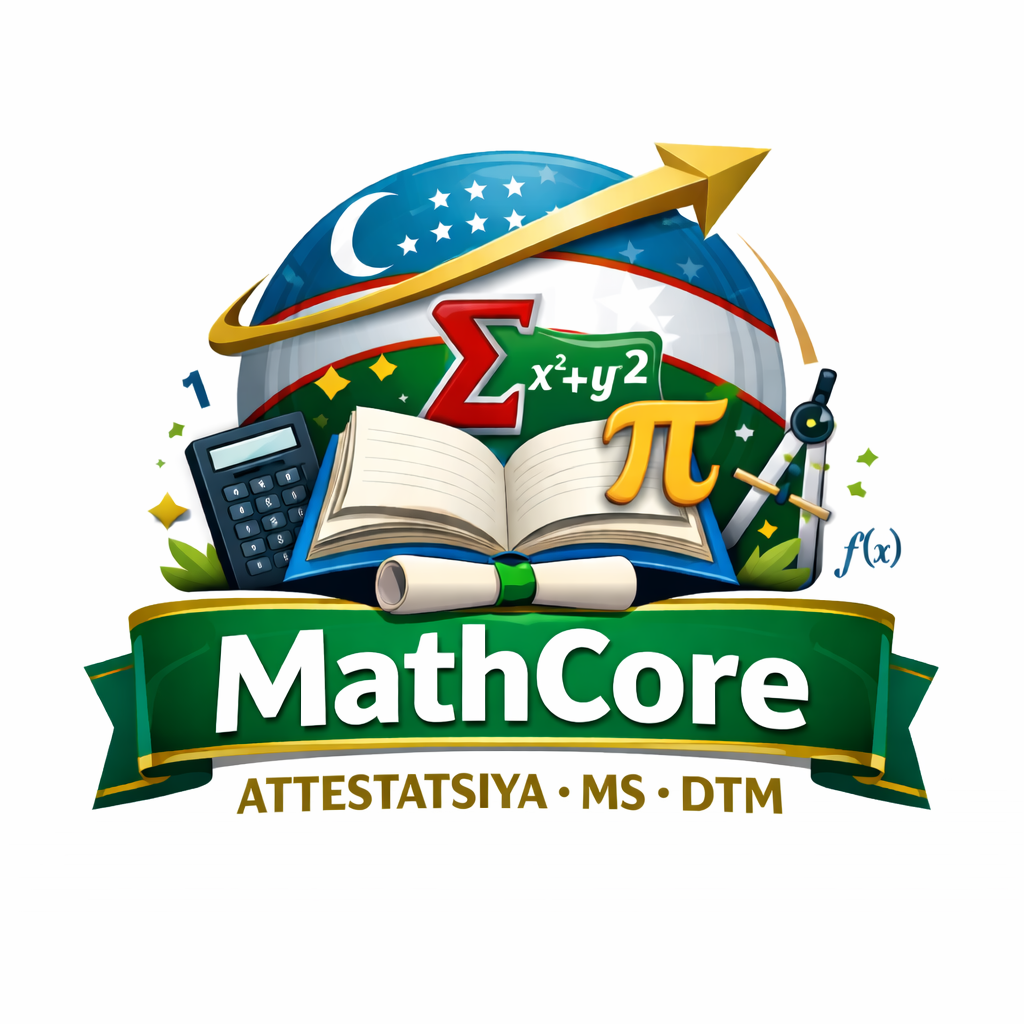
\includegraphics[width=0.2\textwidth]{logo.png} \\[5mm]
    \textcolor{gray}{\small Telegram: \href{https://t.me/Math_Core_Dtm_MS_Att}{@Math\_Core\_Dtm\_MS\_Att}}
\end{center}
\vspace{5mm}
% Задача 1
\begin{questionbox}{1}
    Определите, верны или неверны следующие утверждения:
    \begin{enumerate}
        \item[(I)] \(S_n = \frac{a_1 + a_n}{4} \cdot n\) — формула суммы первых \(n\) членов арифметической прогрессии.
        \item[(II)] Площадь правильного шестиугольника вычисляется по формуле \(S = \frac{3\sqrt{3}a^2}{2}\), где \(a\) — сторона шестиугольника.
        \item[(III)] Производная: \((\arccos x)' = \frac{x}{\sqrt{1-x^2}}\).
    \end{enumerate}
    \begin{options}
        \item I – неверно, II – верно, III – верно
        \item I – неверно, II – верно, III – неверно
        \item I – верно, II – верно, III – верно
        \item I – верно, II – верно, III – неверно
    \end{options}
\end{questionbox}

% Задача 2
\begin{questionbox}{2}
    Число \(a + 2026\) делится без остатка на 10, 12 и 15. Найдите наименьшее натуральное значение \(a\).
    \begin{options}
        \item 14
        \item 8
        \item 6
        \item 4
    \end{options}
\end{questionbox}

% Задача 3
\begin{questionbox}{3}
    Для трёхзначного числа \(\overline{abc}\) и двузначного \(\overline{ac}\) выполнено \(\overline{abc} = 7 \cdot \overline{ac}\). Найдите \(a + b + c\).
    \begin{options}
        \item 6
        \item 7
        \item 10
        \item 13
    \end{options}
\end{questionbox}

% Задача 4
\begin{questionbox}{4}
    В параллелограмме \(ABCD\) проведена биссектриса \(CF\), \(BE \perp AD\). Известно: \(|BC| = 9\), \(|DC| = 13\), \(|BF| = |EF| = x\). Найдите \(x\).
\begin{cc}
        \centering
        
\includegraphics[width=0.5\linewidth]{a.png}
    \end{cc}
        \begin{options}
        \item 3
        \item 4
        \item 5
        \item 6
    \end{options}
\end{questionbox}

% Задача 5
\begin{questionbox}{5}
    Найдите площадь фигуры, заданной системой неравенств:
    \[
    \begin{cases}
        x^2 + y^2 - 2x - 4y \le -1,\\
        3x - 2y + 1 \ge 0.
    \end{cases}
    \]
    \begin{options}
        \item \(2\pi\)
        \item \(3\pi\)
        \item \(4{,}5\pi\)
        \item \(9\pi\)
    \end{options}
\end{questionbox}

% Задача 6
\begin{questionbox}{6}
    Для многочлена \(P(x)\) выполнено \(P(3x+2) = x^2 + ax + 4\). Остаток от деления \(P(x+1)\) на \(x-4\) равен 8. Найдите \(a\).
    \begin{options}
        \item 1
        \item 2
        \item 3
        \item 4
    \end{options}
\end{questionbox}

% Задача 7
\begin{questionbox}{7}
    На полуокружности отмечены 6 точек. Найдите вероятность того, что три случайно выбранные точки не могут быть вершинами треугольника.
\begin{cc}
        \centering
        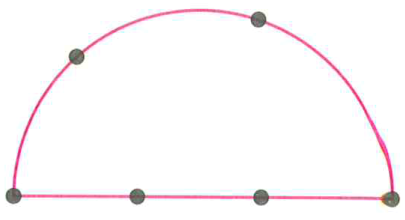
\includegraphics[width=0.5\linewidth]{dsa.png}
    \end{cc}
        \begin{options}
        \item \(\frac{1}{10}\)
        \item \(\frac{1}{5}\)
        \item \(\frac{2}{5}\)
        \item \(\frac{4}{5}\)
    \end{options}
\end{questionbox}

% Задача 8
\begin{questionbox}{8}
    Треугольник \(OAB\) построен на векторах \(\mathbf{a} = \overrightarrow{OA}\) и \(\mathbf{b} = \overrightarrow{OB}\). \(OK\) — биссектриса треугольника. Выразите \(\overrightarrow{OK}\) через \(\mathbf{a}\) и \(\mathbf{b}\).
    \begin{options}
        \item \(\mathbf{a}+\mathbf{b}\)
        \item \(\frac{|\mathbf{b}|\mathbf{a} + |\mathbf{a}|\mathbf{b}}{|\mathbf{a}|+|\mathbf{b}|}\)
        \item \(\frac{|\mathbf{a}|\mathbf{a} + |\mathbf{b}|\mathbf{b}}{|\mathbf{a}|+|\mathbf{b}|}\)
        \item \(\frac{\mathbf{a}}{|\mathbf{a}|} + \frac{\mathbf{b}}{|\mathbf{b}|}\)
    \end{options}
\end{questionbox}

% Задача 9
\begin{questionbox}{9}
    Вычислите \(f(11{,}25^\circ)\), если
    \[
    f(x) = \frac{\sin 6x}{\sin 2x} + \frac{\cos 6x}{\cos 2x}.
    \]
    \begin{options}
        \item 4
        \item \(2\sqrt{2}\)
        \item 0
        \item \(-2\sqrt{2}\)
    \end{options}
\end{questionbox}

% Задача 10
\begin{questionbox}{10}
    Вершина \(B\) равнобедренного треугольника \(OBC\) (\(|OB| = |BC|\)) лежит на параболе \(y = f(x)\), а остальные вершины — на осях \(Oy\) и \(Ox\). При какой абсциссе точки \(B\) площадь треугольника будет наименьшей?
\begin{cc}
        \centering
        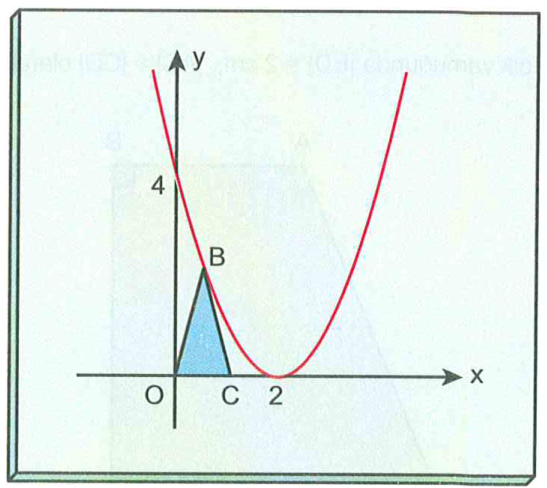
\includegraphics[width=0.5\linewidth]{aswww.png}
    \end{cc}
        \begin{options}
        \item \(\frac{1}{4}\)
        \item \(\frac{1}{3}\)
        \item \(\frac{1}{2}\)
        \item \(\frac{2}{3}\)
    \end{options}
\end{questionbox}

% Задача 11
\begin{questionbox}{11}
    Используя равенство
    \[
    \frac{x^2 + 3x}{x^3 - 2x^2 - 9x + 18} = \frac{x^2 - ax}{x^3 - 3x^2 - 4x + 12},
    \]
    найдите \(a\).
    \begin{options}
        \item 1
        \item \(-3\)
        \item 2
        \item \(-2\)
    \end{options}
\end{questionbox}

% Задача 12
\begin{questionbox}{12}
    Для последовательности \(a_1, a_2, \dots\) выполнено \(a_{n+2} = a_{n+1} + a_n\) (\(n=1,2,\dots\)). Если \(a_7 = 4\), найдите \(a_5 + a_8\).
    \begin{options}
        \item 6
        \item 8
        \item 10
        \item 12
    \end{options}
\end{questionbox}

% Задача 13
\begin{questionbox}{13}
    Для геометрической прогрессии \(\{b_n\}\) известно: \(b_9 - b_1 = 3\), \(b_{12} - b_4 = 24\). Найдите знаменатель прогрессии.
    \begin{options}
        \item \(0{,}(6)\)
        \item \(0{,}5\)
        \item 2
        \item 3
    \end{options}
\end{questionbox}

% Задача 14
\begin{questionbox}{14}
    На рисунке изображены три прямоугольника. \(\angle NLD = 140^\circ\), \(\angle AKE = 100^\circ\). Найдите \(\angle MRF = \alpha\).
\begin{cc}
    \centering
    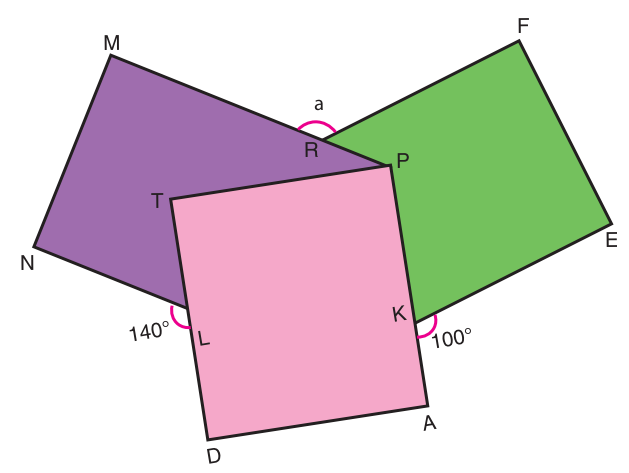
\includegraphics[width=0.5\linewidth]{hg.png}
    \end{cc}
        \begin{options}
        \item \(100^\circ\)
        \item \(110^\circ\)
        \item \(120^\circ\)
        \item \(130^\circ\)
    \end{options}
\end{questionbox}

% Задача 15
\begin{questionbox}{15}
    Пять мастеров выполняют работу за 20 дней, пять учеников — за 30 дней. За сколько дней выполнят эту работу 2 мастера и 2 ученика?
    \begin{options}
        \item 30 дней
        \item 15 дней
        \item 22 дня
        \item 18 дней
    \end{options}
\end{questionbox}

% Задача 16
\begin{questionbox}{16}
    В прямоугольном треугольнике \(ABC\): \(|AE| = |EC|\), \(|BD| = 2\), \(|AD| = 8\), \(|BC| = 6\). Найдите \(\angle ADE = x\).
    \begin{cc}
        \centering
        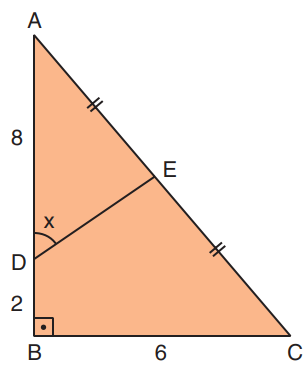
\includegraphics[width=0.3\linewidth]{fafa.png}
    \end{cc}
\begin{figure}
        \centering
        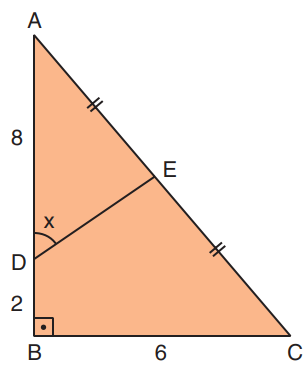
\includegraphics[width=0.5\linewidth]{fg.png}
    \end{figure}
        \begin{options}
        \item \(30^\circ\)
        \item \(45^\circ\)
        \item \(60^\circ\)
        \item \(75^\circ\)
    \end{options}
\end{questionbox}

% Задача 17
\begin{questionbox}{17}
    Вычислите:
    \[
    \frac{\log_2 \sqrt{8} + \log_8 \sqrt{2}}{\log_2 \sqrt{8} - \log_8 \sqrt{2}}.
    \]
    \begin{options}
        \item \(\frac{5}{4}\)
        \item \(\frac{6}{5}\)
        \item \(\frac{7}{6}\)
        \item \(\frac{10}{7}\)
    \end{options}
\end{questionbox}

% Задача 18
\begin{questionbox}{18}
    В прямоугольной трапеции \(ABCD\) высота равна 6, боковая сторона равна большему основанию. При каком значении меньшего основания площадь трапеции будет наименьшей?
    \begin{options}
        \item \(2\sqrt{3}\)
        \item 6
        \item \(3\sqrt{5}\)
        \item 10
    \end{options}
\end{questionbox}

% Задача 19
\begin{questionbox}{19}
    В четырёхугольнике \(ABCD\) из точки \(E\) проведены отрезки к серединам сторон \(K, L, M, N\), разделяющие четырёхугольник на четыре части. Числа внутри кругов обозначают площади. Найдите \(S\).
    \begin{cc}
        \centering
        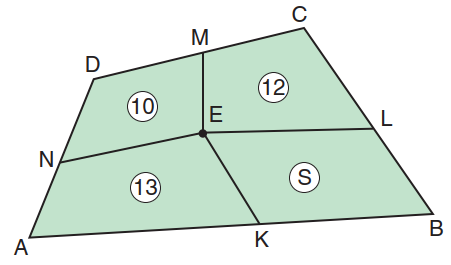
\includegraphics[width=0.5\linewidth]{qda.png}
    \end{cc}
\begin{figure}
        \centering
        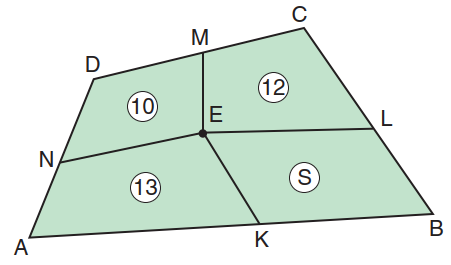
\includegraphics[width=0.5\linewidth]{we.png}
    \end{figure}
        \begin{options}
        \item 12
        \item 13
        \item 14
        \item 15
    \end{options}
\end{questionbox}

% Задача 20
\begin{questionbox}{20}
    Для различных действительных чисел \(m\) и \(n\) выполнено \(n^2 f(m) = m^2 f(n)\). Найдите \(\frac{f(3)-f(1)}{f(4)}\).
    \begin{options}
        \item \(\frac{1}{8}\)
        \item \(\frac{1}{2}\)
        \item \(\frac{5}{8}\)
        \item \(\frac{3}{4}\)
    \end{options}
\end{questionbox}

% Задача 21
\begin{questionbox}{21}
    Пусть
    \[
    f(x) = \frac{1}{x} + \frac{1}{x^2} + \frac{1}{x^3} + \dots + \frac{1}{x^n}.
    \]
    Если \(f'(1) = -66\), найдите \(n\).
    \begin{options}
        \item 9
        \item 10
        \item 11
        \item 12
    \end{options}
\end{questionbox}

% Задача 22
\begin{questionbox}{22}
    Два насоса одинаковой мощности заполняют бассейн за 20 часов. Если мощность первого уменьшить на 20\%, а мощность второго увеличить на 60\%, за сколько часов заполнится бассейн?
    \begin{options}
        \item 35
        \item 30
        \item 32
        \item \(\frac{50}{3}\)
    \end{options}
\end{questionbox}

% Задача 23
\begin{questionbox}{23}
    В трапеции \(ABCD\) отрезок \(EF\) — средняя линия. \(S_{ETK} : S_{KF} = 3 : 2\). Найдите \(KF : EK\).
\begin{cc}
        \centering
        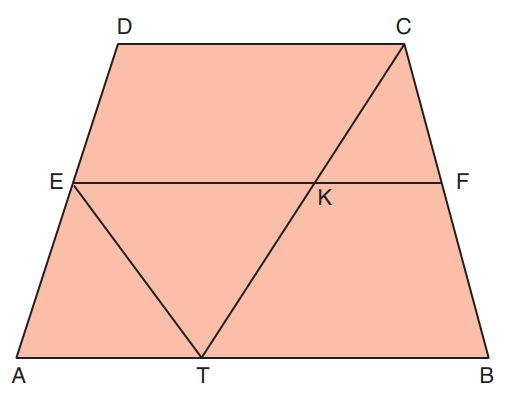
\includegraphics[width=0.3\linewidth]{rew.png}
    \end{cc}
        \begin{options}
        \item \(\frac{3}{2}\)
        \item \(\frac{4}{3}\)
        \item \(\frac{2}{3}\)
        \item \(\frac{3}{4}\)
    \end{options}
\end{questionbox}

% Задача 24
\begin{questionbox}{24}
    Решите неравенство:
    \[
    \log_{\frac{1}{3}} \bigl( \log_2 (2 - x) \bigr) + 1 \ge 0.
    \]
    \begin{options}
        \item \([-6; 1)\)
        \item \([-6; 2)\)
        \item \([-6; 2) \cup (2; \infty)\)
        \item \((1; 2)\)
    \end{options}
\end{questionbox}

% Задача 25
\begin{questionbox}{25}
    Если \(f(x) = -\dfrac{2}{x}\), найдите функцию \(y = f(x+2) + 1\).
    \begin{options}
        \item \(y = -\dfrac{x}{x+2}\)
        \item \(y = \dfrac{1}{x+2}\)
        \item \(y = \dfrac{2x}{x+2}\)
        \item \(y = \dfrac{x}{x+2}\) 
    \end{options}
\end{questionbox}
% Задача 26
\begin{questionbox}{26}
    Решите неравенство на отрезке \([0; \pi]\):
    \[
    \sin^2 x < \cos^2 x - \frac{\sqrt{3}}{2}.
    \]
    \begin{options}
        \item \(\left[0; \frac{\pi}{12}\right) \cup \left(\frac{11\pi}{12}; \pi\right]\)
        \item \(\left(\frac{\pi}{12}; \frac{11\pi}{12}\right)\)
        \item \(\left[0; \frac{5\pi}{12}\right]\)
        \item \(\left[0; \pi\right]\)
    \end{options}
\end{questionbox}

% Задача 27
\begin{questionbox}{27}
    В параллелограмме \(ABCD\): \(|EF| = |FB|\), \(|DF| = |FT| = |TC|\), \(|CL| = |LB|\). Площадь жёлтой области равна 8. Найдите площадь синей области.
\begin{cc}
        \centering
        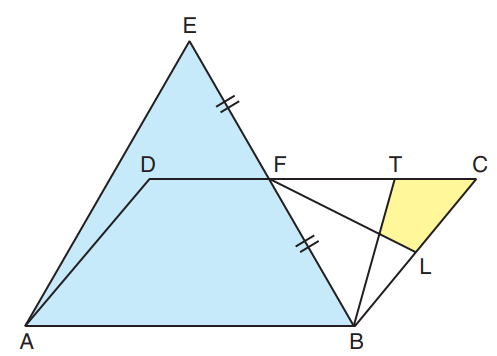
\includegraphics[width=0.5\linewidth]{равр.png}
    \end{cc}
        \begin{options}
        \item 72
        \item 60
        \item 48
        \item 36
    \end{options}
\end{questionbox}

% Задача 28
\begin{questionbox}{28}
    Решите уравнение \(2\sin^2\left(x + \frac{\pi}{6}\right) + 3\sin\left(x + \frac{\pi}{6}\right) - 2 = 0\) и укажите его наименьший положительный корень.
    \begin{options}
        \item \(\frac{\pi}{6}\)
        \item \(\frac{\pi}{4}\)
        \item \(\frac{2\pi}{3}\)
        \item \(\frac{3\pi}{4}\)
    \end{options}
\end{questionbox}

% Задача 29
\begin{questionbox}{29}
    В треугольнике \(ABC\) \(BD\) — биссектриса, \(|BE| = 3|ED| = 9\). Найдите \(|DC| = x\).
\begin{cc}
        \centering
        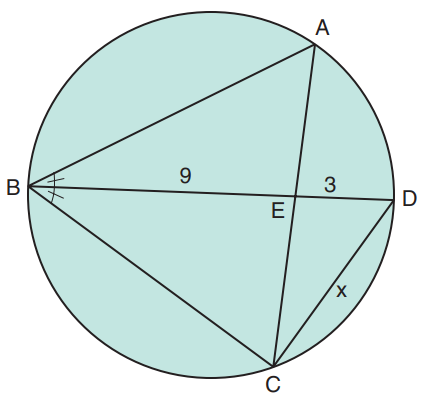
\includegraphics[width=0.5\linewidth]{fafw.png}
    \end{cc}
        \begin{options}
        \item 9
        \item 8
        \item 7
        \item 6
    \end{options}
\end{questionbox}

% Задача 30
\begin{questionbox}{30}
    Согласно схеме, сколькими различными способами можно попасть из точки \(A\) в точку \(C\)?
\begin{cc}
        \centering
        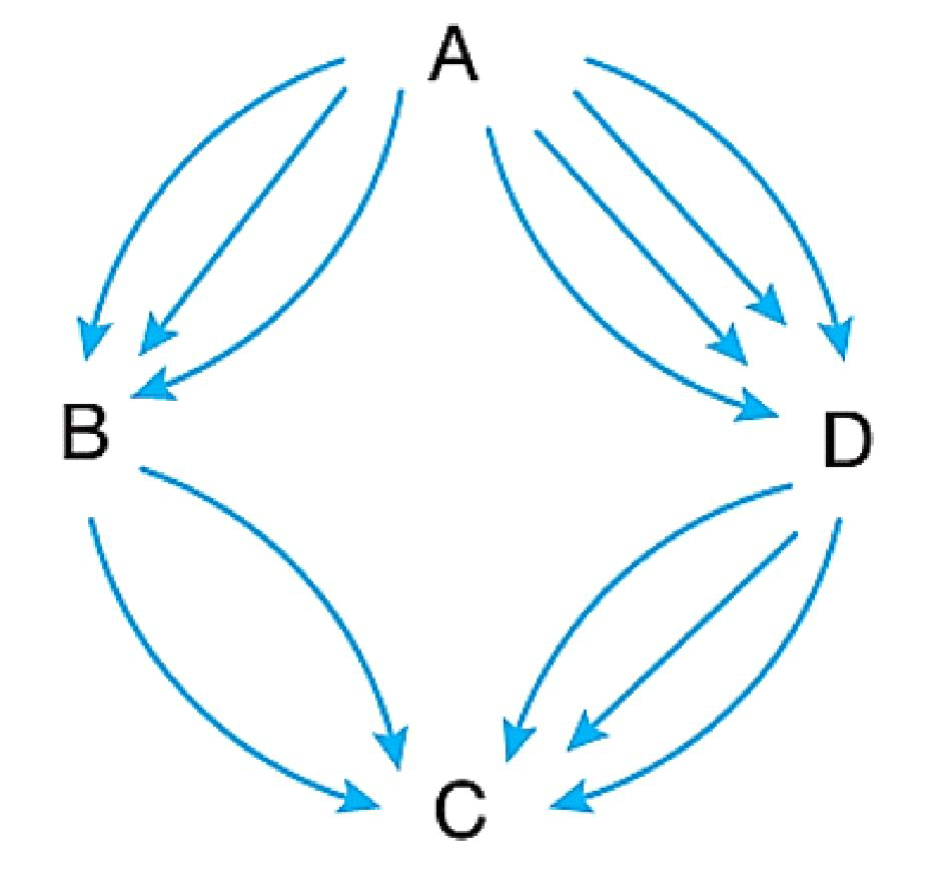
\includegraphics[width=0.5\linewidth]{ert.png}
    \end{cc}
        \begin{options}
        \item 12
        \item 14
        \item 16
        \item 18
    \end{options}
\end{questionbox}

% Задача 31
\begin{questionbox}{31}
    Правильный шестиугольник \(ABCDEF\) со стороной 4. Внутри него проведены дуги окружностей с центрами в вершинах шестиугольника. Найдите площадь зелёной области.
\begin{cc}
        \centering
        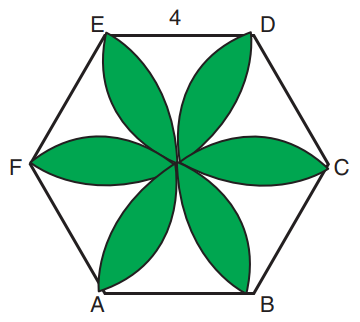
\includegraphics[width=0.5\linewidth]{232er.png}
    \end{cc}
        \begin{options}
        \item \(16\pi - 32\sqrt{3}\)
        \item \(32\pi - 36\sqrt{3}\)
        \item \(24\pi - 32\sqrt{3}\)
        \item \(32\pi - 48\sqrt{3}\)
    \end{options}
\end{questionbox}

% Задача 32
\begin{questionbox}{32}
    Вычислите неопределённый интеграл:
    \[
    \int 4x \cdot \ln(3x) \, dx.
    \]
    \begin{options}
        \item \(2x^2 \ln(3x) - x^2 + C\)
        \item \(x^2 \ln(3x) - 2x^2 + C\)
        \item \(2x^2 \ln(3x) - 2x^2 + C\)
        \item \(4x^2 \ln(3x) - x^2 + C\)
    \end{options}
\end{questionbox}

% Задача 33
\begin{questionbox}{33}
    На рисунке изображены параллельные доски банного оборудования. Уравнения прямых, на которых лежат первая, вторая и третья доски: \(d_1\), \(d_2\), \(d_3\). Найдите отношение расстояния между \(d_1\) и \(d_2\) к расстоянию между \(d_2\) и \(d_3\).
\begin{cc}
        \centering
        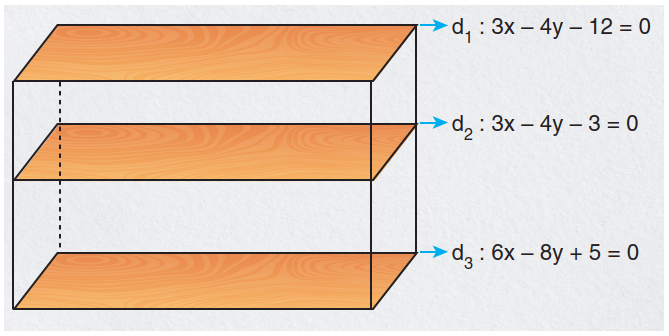
\includegraphics[width=0.5\linewidth]{tw.png}
    \end{cc}
        \begin{options}
        \item \(\frac{10}{11}\)
        \item \(\frac{12}{11}\)
        \item \(\frac{16}{11}\)
        \item \(\frac{18}{11}\)
    \end{options}
\end{questionbox}

% Задача 34
\begin{questionbox}{34}
    На чертеже \(|AB| = 5\), \(|BC| = 6\), \(|EF| = 2\), \(|FG| = 3\). Красный картон вращается на \(360^\circ\) вокруг прямой \(d\). Найдите объём полученного тела.
\begin{cc}
        \centering
        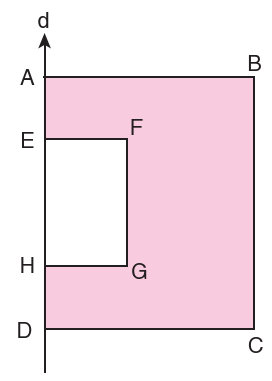
\includegraphics[width=0.4\linewidth]{5tr.png}
    \end{cc}
        \begin{options}
        \item \(148\pi\)
        \item \(168\pi\)
        \item \(138\pi\)
        \item \(128\pi\)
    \end{options}
\end{questionbox}

% Задача 35
\begin{questionbox}{35}
    Корни многочлена \(10x^3 - 39x^2 + 29x - 6\) равны длине, ширине и высоте прямоугольного параллелепипеда. Каждое ребро параллелепипеда увеличили на 2 единицы. Найдите объём получившегося параллелепипеда.
    \begin{options}
        \item 20
        \item 24
        \item 30
        \item 36
    \end{options}
\end{questionbox}

\end{document}